\section{Nome do Jogo} Ogof e o templo das joias.

\section{\textit{High Concept} do Jogo} Ogof e o templo das joias é um game de
fantasia, em que o jogador assumirá o papel de 3 diferentes figuras, e trabalhar
em conjunto para progredir.

\section{Gênero}
Com o avanço da tecnologia, os jogos passar a ficar cada vez mais complexos, e dessa forma, passam a abrigar diversos gêneros e sub-gêneros em um único titulo, em \textbf{Ogof e o templo das Joias} optou-se por utilizar dois gêneros, para que se potencializasse a "rejogabilidade", conceito do inglês \textit{replay value}, ou \textit{replayability}, que mensura a disposição de um jogador, se manter jogando, mesmo depois de ter finalizado o jogo.

Ação-aventura, em que um personagem deve travar diversas batalhas enquanto explora um ambiente, foi um dos mais sucedidos na industria de jogos, por essa razão originaram-se diversos "sub gêneros', dentre estes, temos o \textit{Hack n' Slash}, que foca a mecânica do jogo no combate, seja ele corpo a corpo seja a distância, God of War, que e possível ver na sessão Inspirações, foi um dos grande títulos que disseminaram este subgênero.

Além do combate, o projeto conterá elementos de resolução de \textit{puzzles} ou em português quebra-cabeças, sendo assim, o jogador devera utilizar habilidades seu raciocínio logico e reconhecimento de padrões para avançar no jogo e desbloquear novas áreas.

\section{Púbico Alvo}

Quando observa-se a produção de entretenimento juvenil, seja em livros, series ou filmes, percebe-se a presença de títulos que abordam a fantasia e elementos fantásticos, tal com Harry Potter, Eragon, entre outros títulos. Como o projeto aborda esses elementos definiu-se o publico alvo para jovens, de ambos os sexos, a partir dos doze anos.

O projeto faz uso de imagem lalala, assim assim assado que, e segundo o manual de classificação do brasil, deve ser classificado como XPTO, o que condiz com o publico alvo selecionado.

\section{\textit{Game Flow}}

O Gráfico de \textit{Game flow} apresenta os possíveis caminhos de telas de um jogo, abaixo, conseguimos observar de forma simplificada, que ao iniciar o jogo, será mostrado os logos, da engine, da FATEC SCS, e por fim do grupo, assim que terminar de mostra-los, será apresentada a tela de menu, com suas opções, sendo elas, sair do jogo, visualizar os créditos, inciar um novo jogo ou ainda carregar um estado salvo. Esta ultima opção, ao terminar o carregamento ele poderá ser levado a qualquer uma das areas do jogo.
Durante o jogo, tem-se a opção de pausa-lo e voltar para a tela de menu inicial.


\begin{figure}[!htb]
    \caption{\label{fig_grafico}Fluxo de telas} \begin{center}
    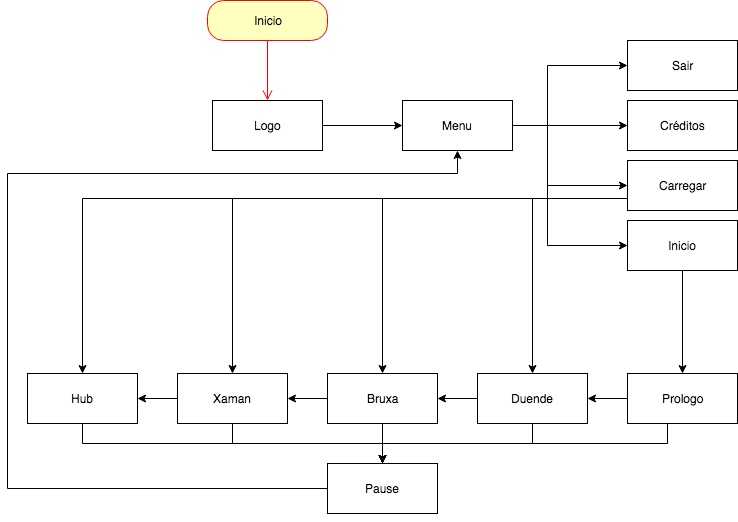
\includegraphics[width=\textwidth]{imagens/Flow.png} \end{center}
\legend{Fonte: Própria Autoria} \end{figure}

\section{Estilo estético}
O jogo será desenvolvido em 3D, utilizando-se a técnica conhecida como \textit{low poly}, que consiste em manter uma baixa contagem de polígonos na modelagem do jogo, segundo Ethan Redd \footnote{Ethan Redd é Game Developer Independente, e paletrante da Game Developers Conference de 2017}, não existe uma delimitação forte para o que é considerado \textit{low poly}, mas ele define de forma não pragmática um modelo que tenha uma contagem menor que oito mil polígonos, ele ainda diz que existem uma série de vantagens em utilizar-se desse estilo estético, como maior produtividade e eficiência computacional, que fazem grande diferença quando se trabalha em times enxutos.

\begin{figure}[htb]
    \caption{\label{fig_lowpoly}Low Poly}
    \begin{center}
        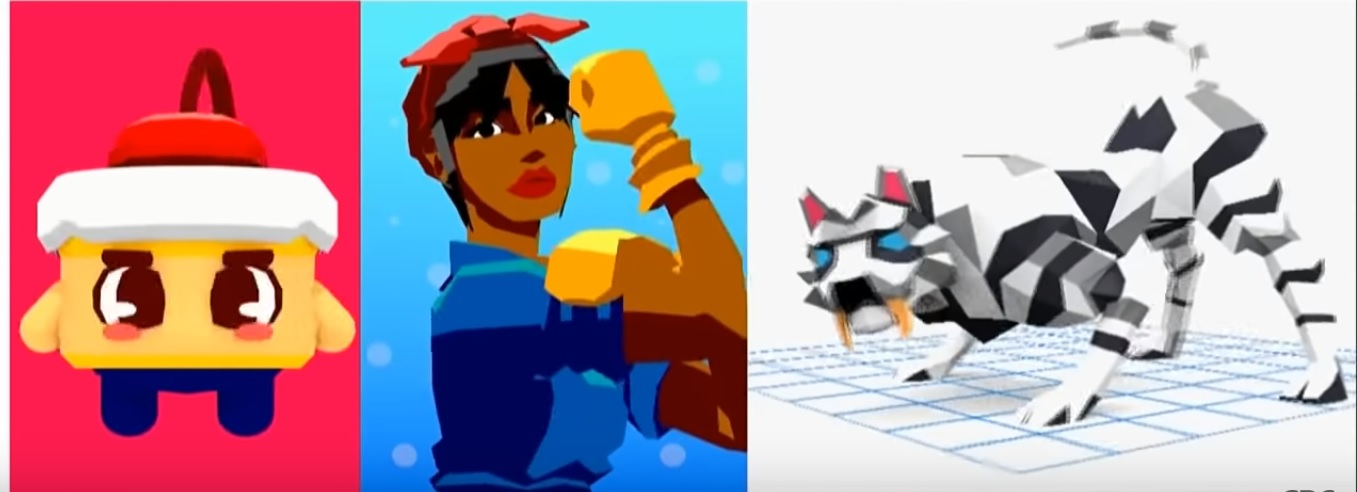
\includegraphics[width=\textwidth]{imagens/lowPoly.jpg}
    \end{center}
    \legend{Fonte: Visite Noruega}
\end{figure}

Dito isso, cada uma das fases do jogo pretende retratar de forma aproximada os ambientes de origem dos personagens, dessa forma a paleta de cores e e objetos encontrados em cada parte do jogo fará alusão a isso.

O mundo do Duende, ou Fulkominn, que quer dizer perfeição em islandês \footnote{Segundo o site https://uwdc.library.wisc.edu/collections/IcelOnline/}, foi baseada na vila de Geiranger da Noruega, que é uma pequena vila incrustada em um fiorde, com uma floresta a abraçando.

\clearpage

\begin{figure}[htb]
    \caption{\label{fig_mundoDuende}Geiranger - Noruega}
    \begin{center}
        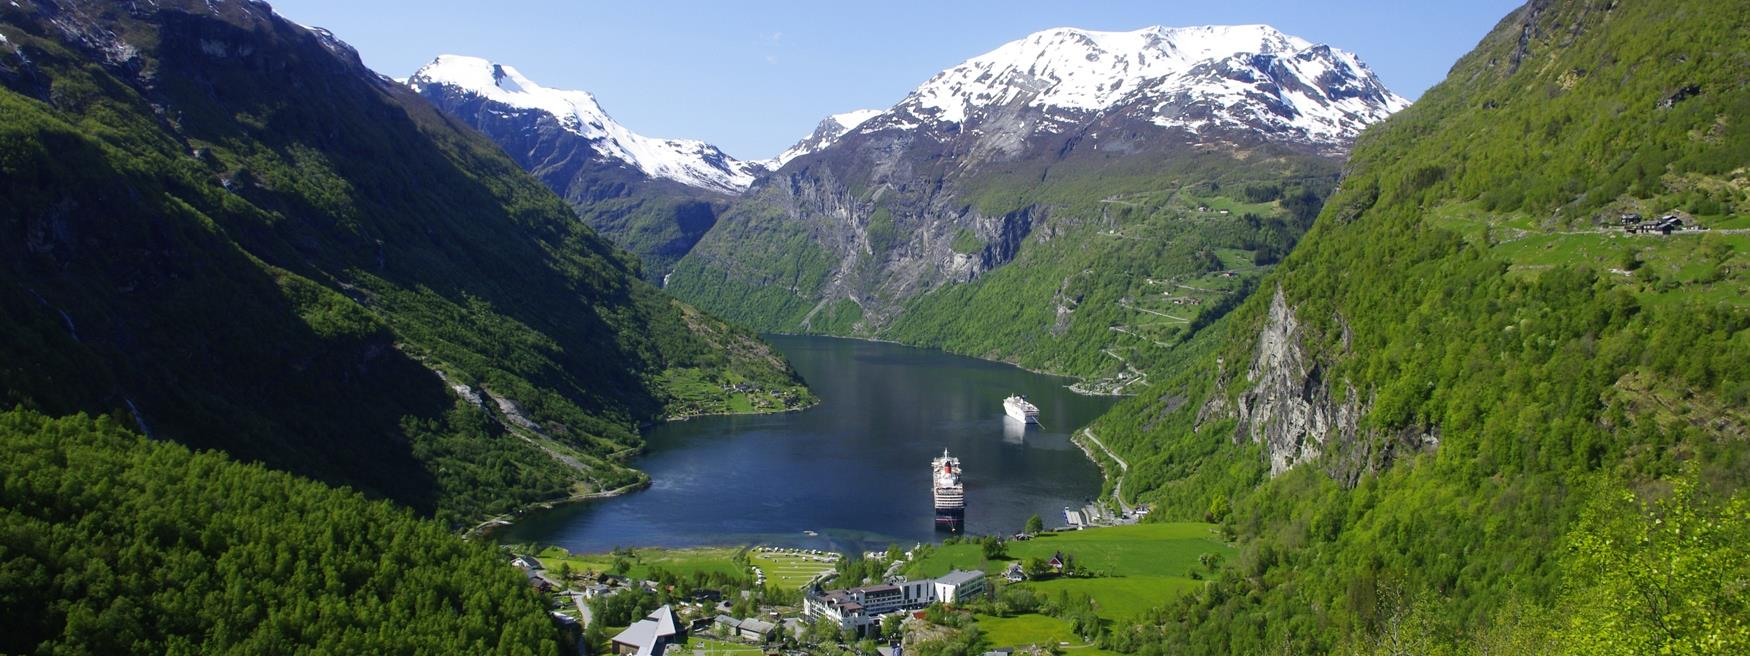
\includegraphics[width=\textwidth]{imagens/geiranger.jpeg}
    \end{center}
    \legend{Fonte: Visite Noruega}
\end{figure}



O mundo da bruxa, foi baseado na cidade de Kilin no Reino Unido, um pequeno vilarejo que se ergue em uma planície escocesa,e desemboca em um lago.

\begin{figure}[htb]
    \caption{\label{fig_mundoBruxa}Kilin - Reino Unido}
    \begin{center}
        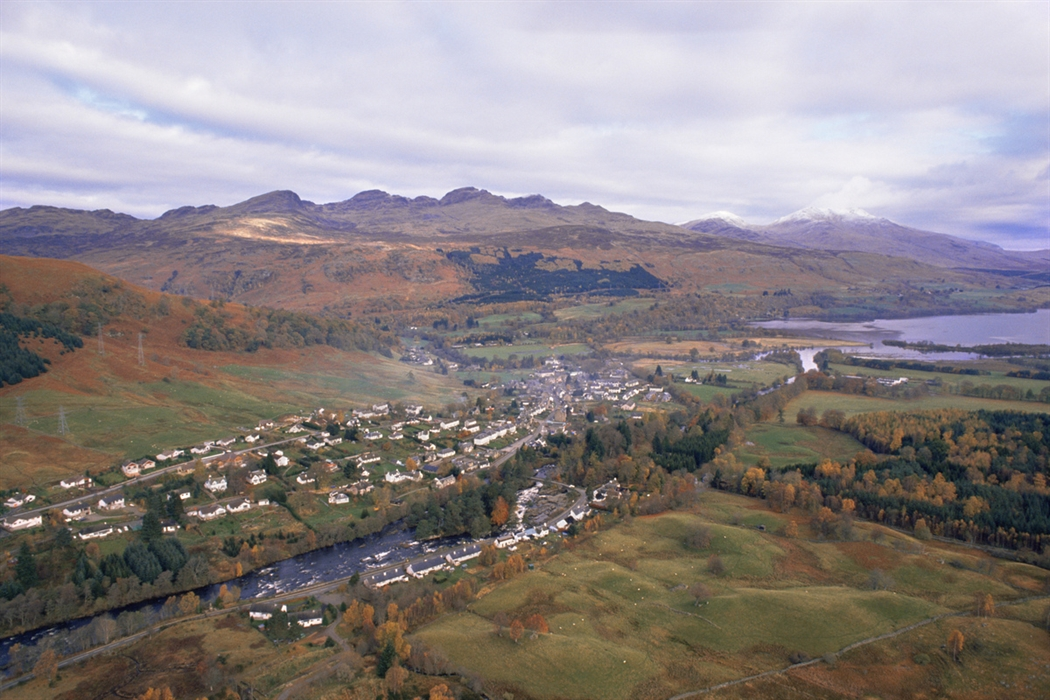
\includegraphics[width=0.9\textwidth]{imagens/kilin.jpg}
    \end{center}
    \legend{Fonte: Visite Noruega}
\end{figure}

\clearpage

O mundo do xamã foi inspirado pelos lugares em que os Pueblos ou Anasazi, viviam, tendo maior inspiração no parque nacional de mesa verde nos estados unidos.


\begin{figure}[htb]
    \caption{\label{fig_mundoXaman}Mesa Verde - Estados Unidos}
    \begin{center}
        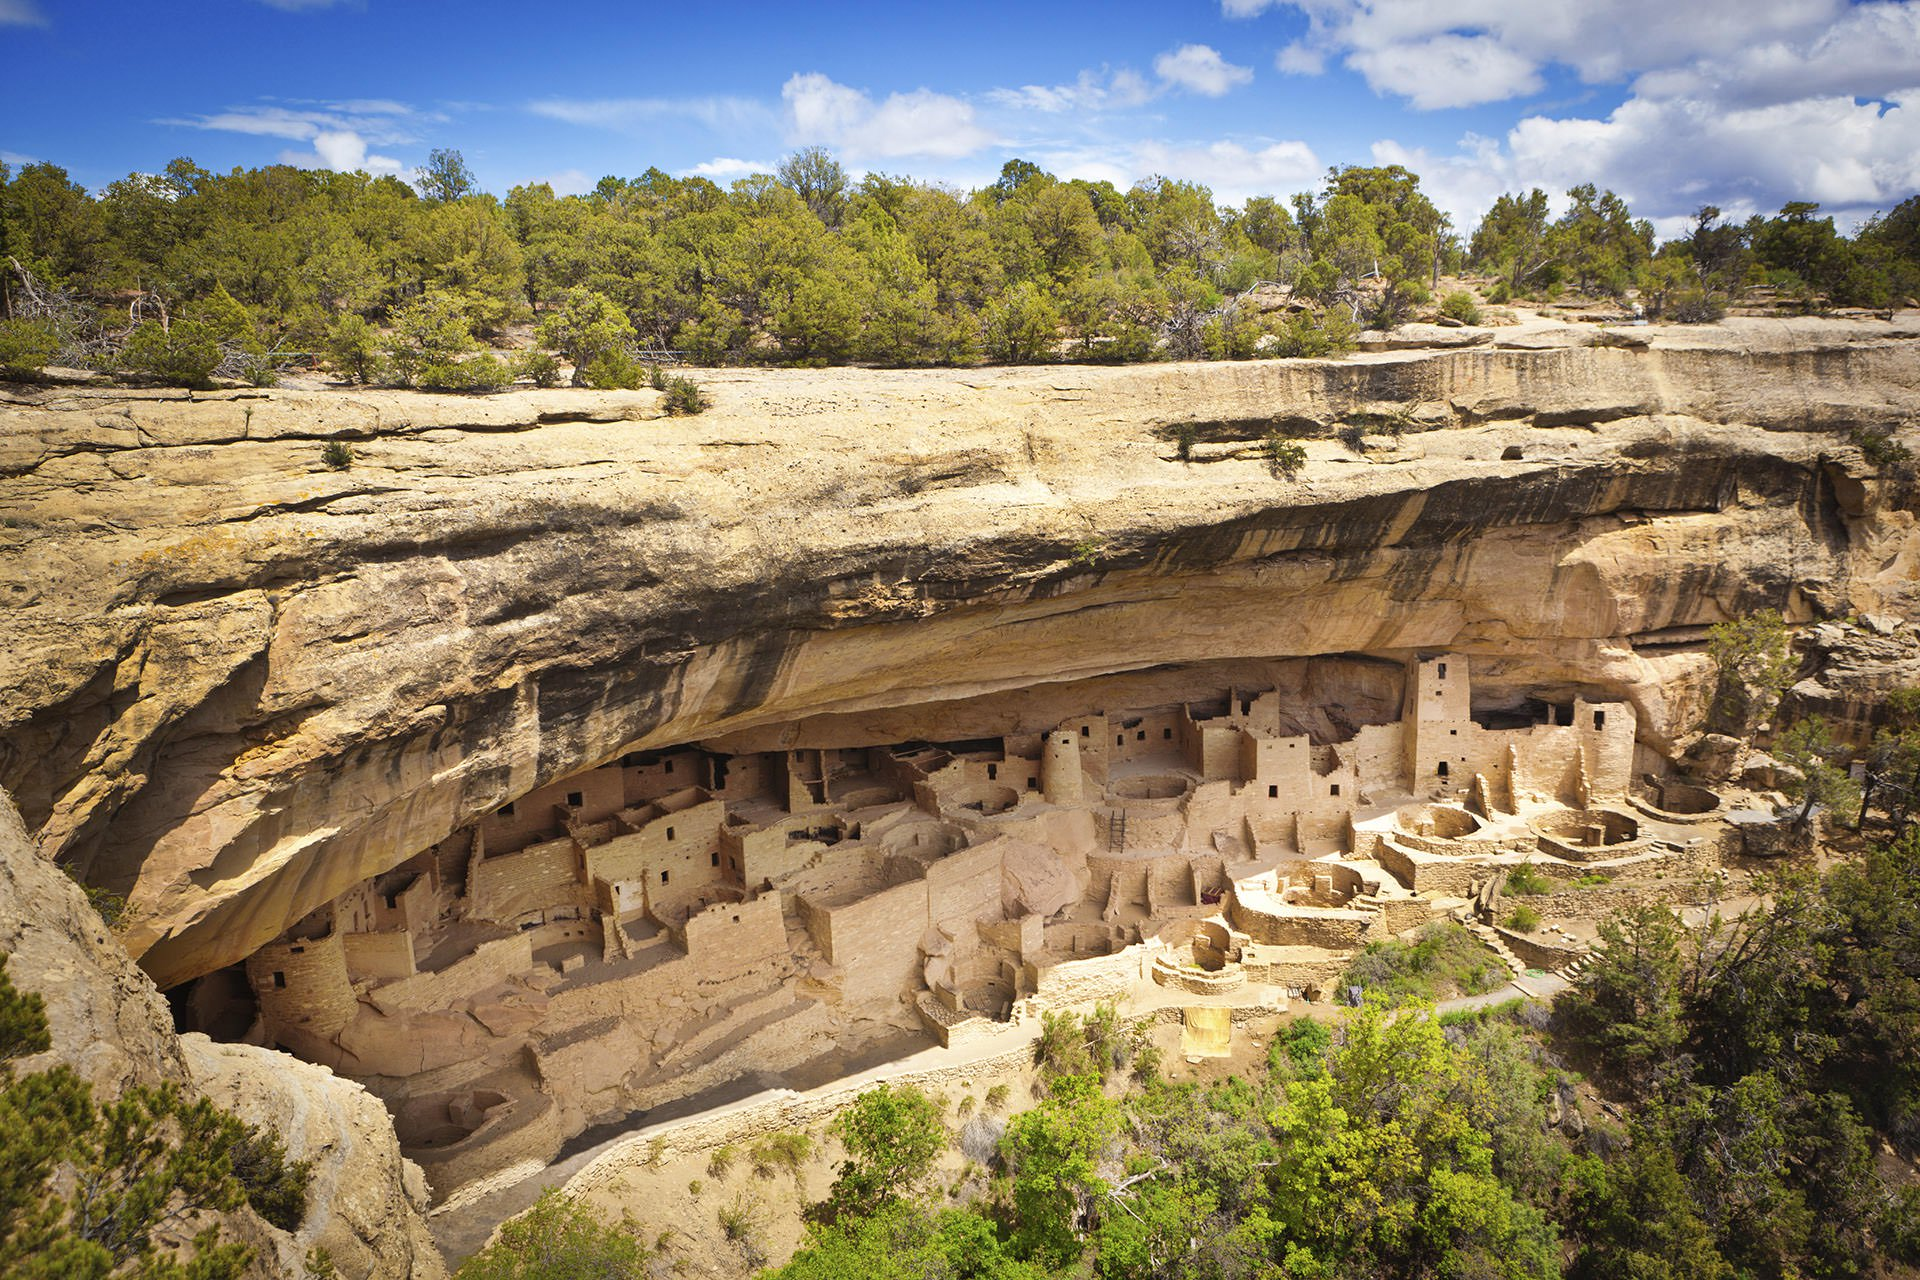
\includegraphics[width=\textwidth]{imagens/mesaverde.jpg}
    \end{center}
    \legend{Fonte: Visite Noruega}
\end{figure}

E por fim, a fase em que todos os elemento se unem, foi baseada no parque nacional de Tikal na Guatemala, antiga formação de um templo Maia.

\clearpage

\begin{figure}[htb]
    \caption{\label{fig_mundoHub}Tikal - Guatemala}
    \begin{center}
        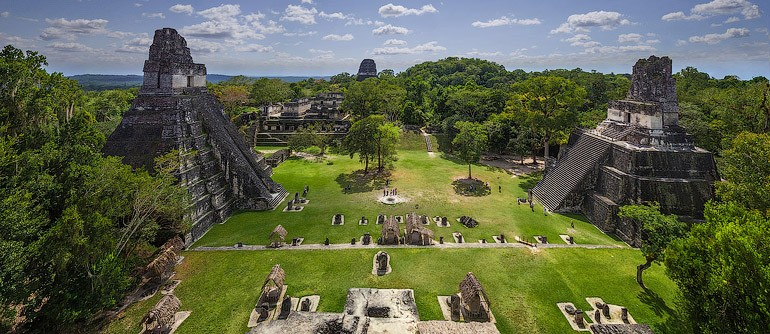
\includegraphics[width=\textwidth]{imagens/tikal.jpg}
    \end{center}
    \legend{Fonte: Visite Noruega}
\end{figure}


\section{Inspirações}


\subsection{Outlander}

Em 1945, em lua de mel na Escócia, a enfermeira em combate Claire Randall é
misteriosamente transportada através do tempo para o ano de 1743.

\begin{figure}[!htb] \caption{\label{Outlander}Outlander} \begin{center}
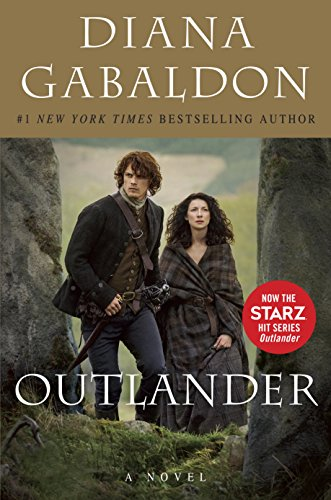
\includegraphics[width=0.3\textwidth]{imagens/outlander.jpg} \end{center}
\legend{Fonte: (Diana Gabaldon, 1991)} \end{figure}

\clearpage

\subsection{Filha de Feiticeira}

Este romance de Celia Rees narra, em forma de diário, a história de Mary
Nuttall, uma adolescente inglesa do século XVII que se vê obrigada a fugir para
a América para não ter o mesmo destino de sua avó, condenada à forca sob
acusação de feitiçaria.

\begin{figure}[!htb] \caption{\label{filha_feiticeira}Filha de Feiticeira}
    \begin{center}
    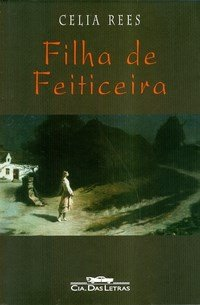
\includegraphics[width=0.3\textwidth]{imagens/feiticeira.jpeg} \end{center}
\legend{Fonte: Celia Rees, 2002} \end{figure}



\subsection{Desencanto}

Bean é uma princesa que vive no reino mágico de Dreamland ao lado de Luci, seu
demônio pessoal, e de Elfo, seu melhor amigo que a acompanham em sua jornada de
alcoolismo, brigas de bar e descobertas inusitadas.



\begin{figure}[!htb] \caption{\label{Desencanto}Desencanto} \begin{center}
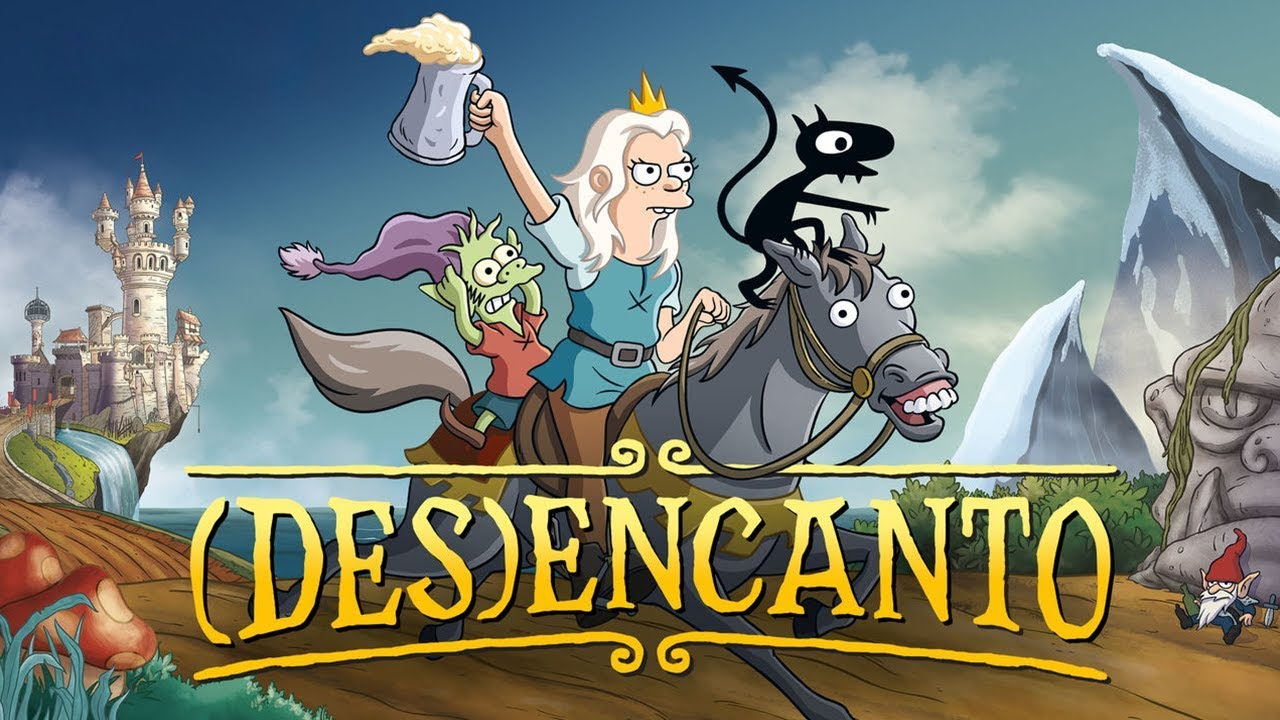
\includegraphics[width=0.5\textwidth]{imagens/Desencanto.jpg} \end{center}
\legend{Fonte: \cite{dessencanto}} \end{figure}

\subsection{Os Vingadores - Guerra infinita}

Neste filme da série Vingadores, os heróis enfrentam Thanos, que pretende juntar
as joias do infinito para prosseguir com seu plano.

\begin{figure}[!htb] \caption{\label{vingadores}Poster do Filme} \begin{center}
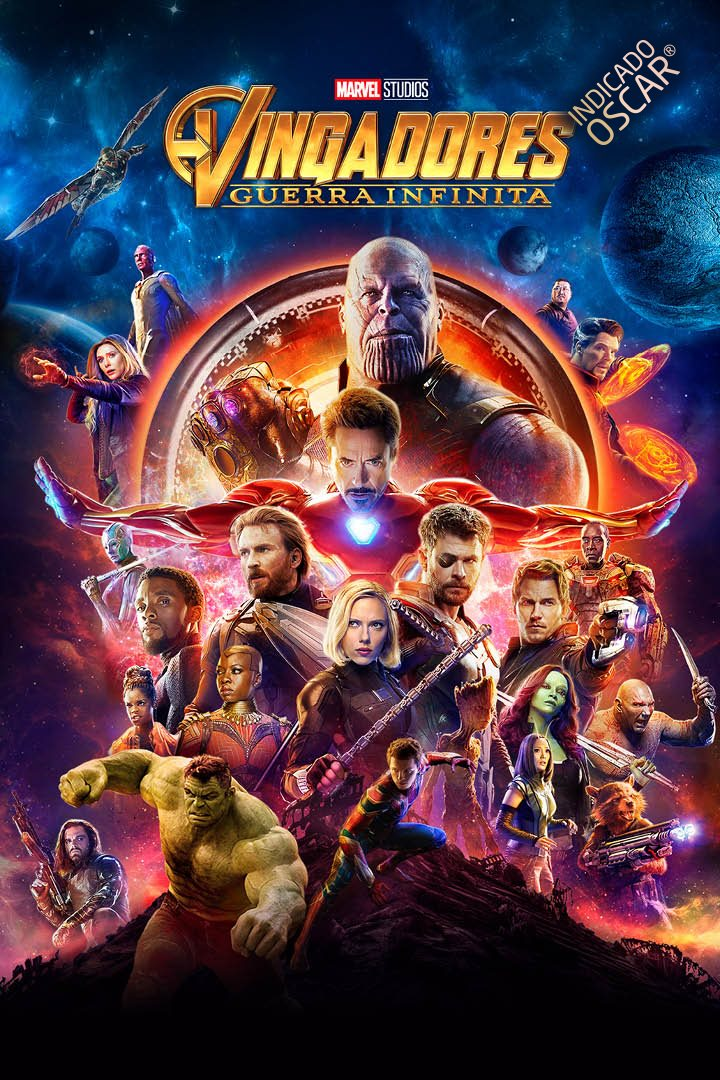
\includegraphics[width=0.3\textwidth]{imagens/vingadores.jpeg} \end{center}
\legend{Fonte: \cite{avengers}} \end{figure}

\subsection{Franquia God of War}

Franquia centrada no personagem Kratos, que foi enganado pelos Deuses e busca
vingança por isso.


\clearpage

\begin{figure}[!htb] \caption{\label{god_of_war}God of War} \begin{center}
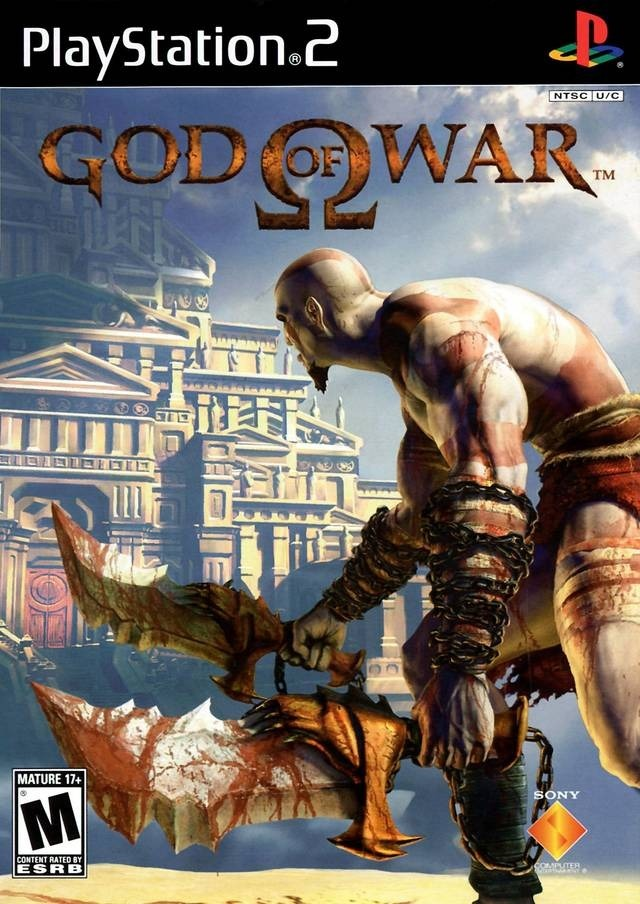
\includegraphics[width=0.3\textwidth]{imagens/GodofWar.jpg} \end{center}
\legend{Fonte: \cite{godofwar}} \end{figure}


\subsection{Brownies}

Brownies são pequenos seres noturnos do folclore britânico, que cuidam dos
afazeres da casa, se ofendem facilmente e evitam serem vistos pelos humanos
\cite{britannica_2011}\cite{carolyn_2016}.

\begin{figure}[!htb]
    \caption{\label{fig_brownie}\textbf{Brownie} por Arthur Rackham }
    \begin{center} 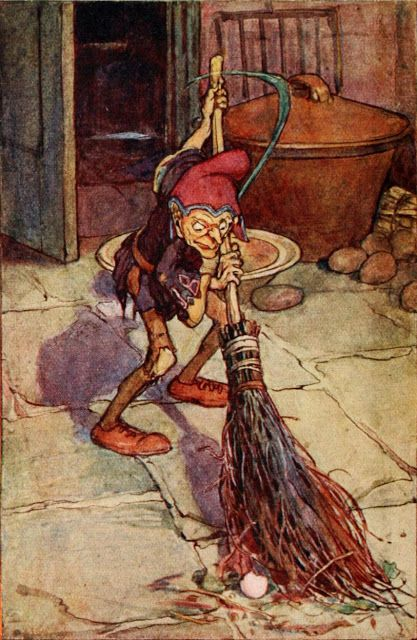
\includegraphics[width=0.3\textwidth]{imagens/brownie.jpg}
    \end{center} \legend{Fonte: \cite{carolyn_2016}} \end{figure}


\subsection{Alux}

Alux são pequenas criaturas da mitologia de alguns povos Maias, costumeiramente
são invisíveis, mas podem se tornar visíveis para se comunicar e assustar
humanos. Segundo Storniolo (\citeyear{storniolo2009out}) ``When given food,
drink, and ritual homage, the aluxo'b protect the farmer’s crops from hungry
animals. [\ldots] The aluxo'b summon strong winds, emit piercing whistling
sounds, and propel stones at intruders.'' [Quando recebem comida, bebida e
um ritual de homenagem, o alux protegerá a plantação do fazendeiro de
animais famintos. [\ldots] O alux invoca fortes ventos, emite agudos sons
sibilantes, e lança pedras em instrusos: tradução livre]


\begin{figure}[!htb] \caption{\label{fig_alux}Alux} \begin{center}
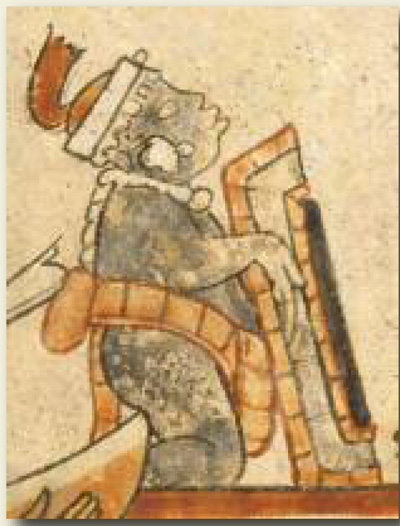
\includegraphics[width=0.3\textwidth]{imagens/alux.jpg} \end{center}
\legend{Fonte:~\cite{storniolo2009out}} \end{figure}

\subsection{Pueblos}

Pueblos foi  um povo que habitou o que hoje é o sudoeste dos Estados Unidos,
mais especificamente a região de Colorado, Utah, Novo México, e
Arizona.\cite{civPerdidas2017,lyneis1995virgin}
Acredita-se que são antepassados de diversas tribos norte americanas como Ute,
Zuni, Navajo e Hopi, e que essas tribos ainda pratiquem seus rituais. Pela
região que habitam, grande parte de seus ritos ocorriam para os deuses da
chuva\cite{abreu94}.

\clearpage

\begin{figure}[!htb] \caption{\label{fig_puebloan}Construção Pueblo} \begin{center}
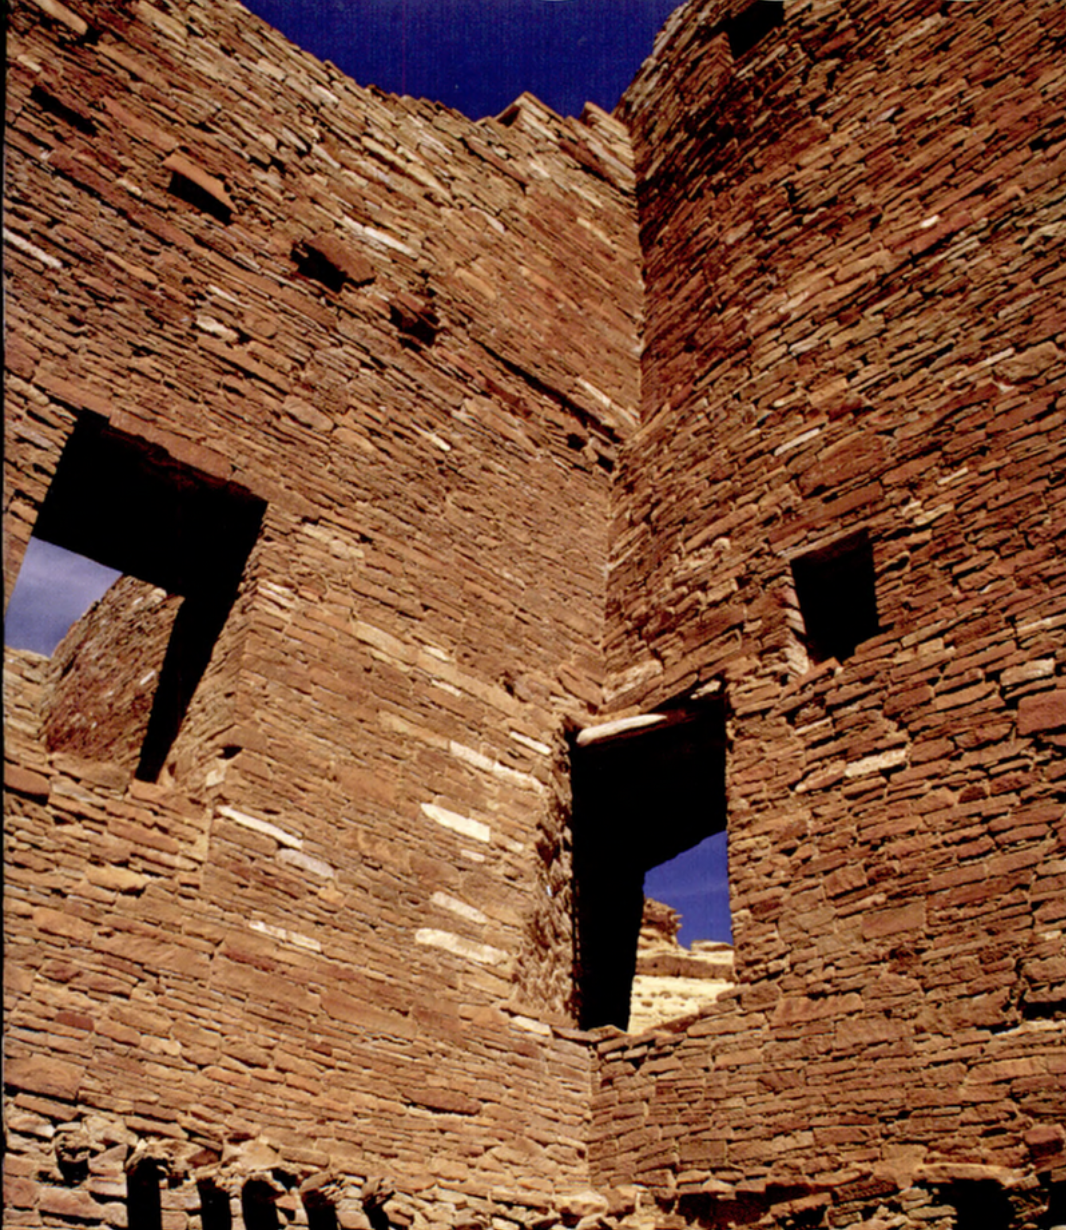
\includegraphics[width=0.5\textwidth]{imagens/puebloans.png} \end{center}
\legend{Fonte:~\cite{heyder1997anasazi}} \end{figure}


\subsection{Siempre Bruja}

A série que conta a história de uma bruxa negra e escrava que é transportada
pelo tempo para enfrentar um grande bruxo inspirou os poderes da bruxa e itens
com os quais trabalha.

\begin{figure}[!htb] \caption{\label{siempre}Siempre Bruja} \begin{center}
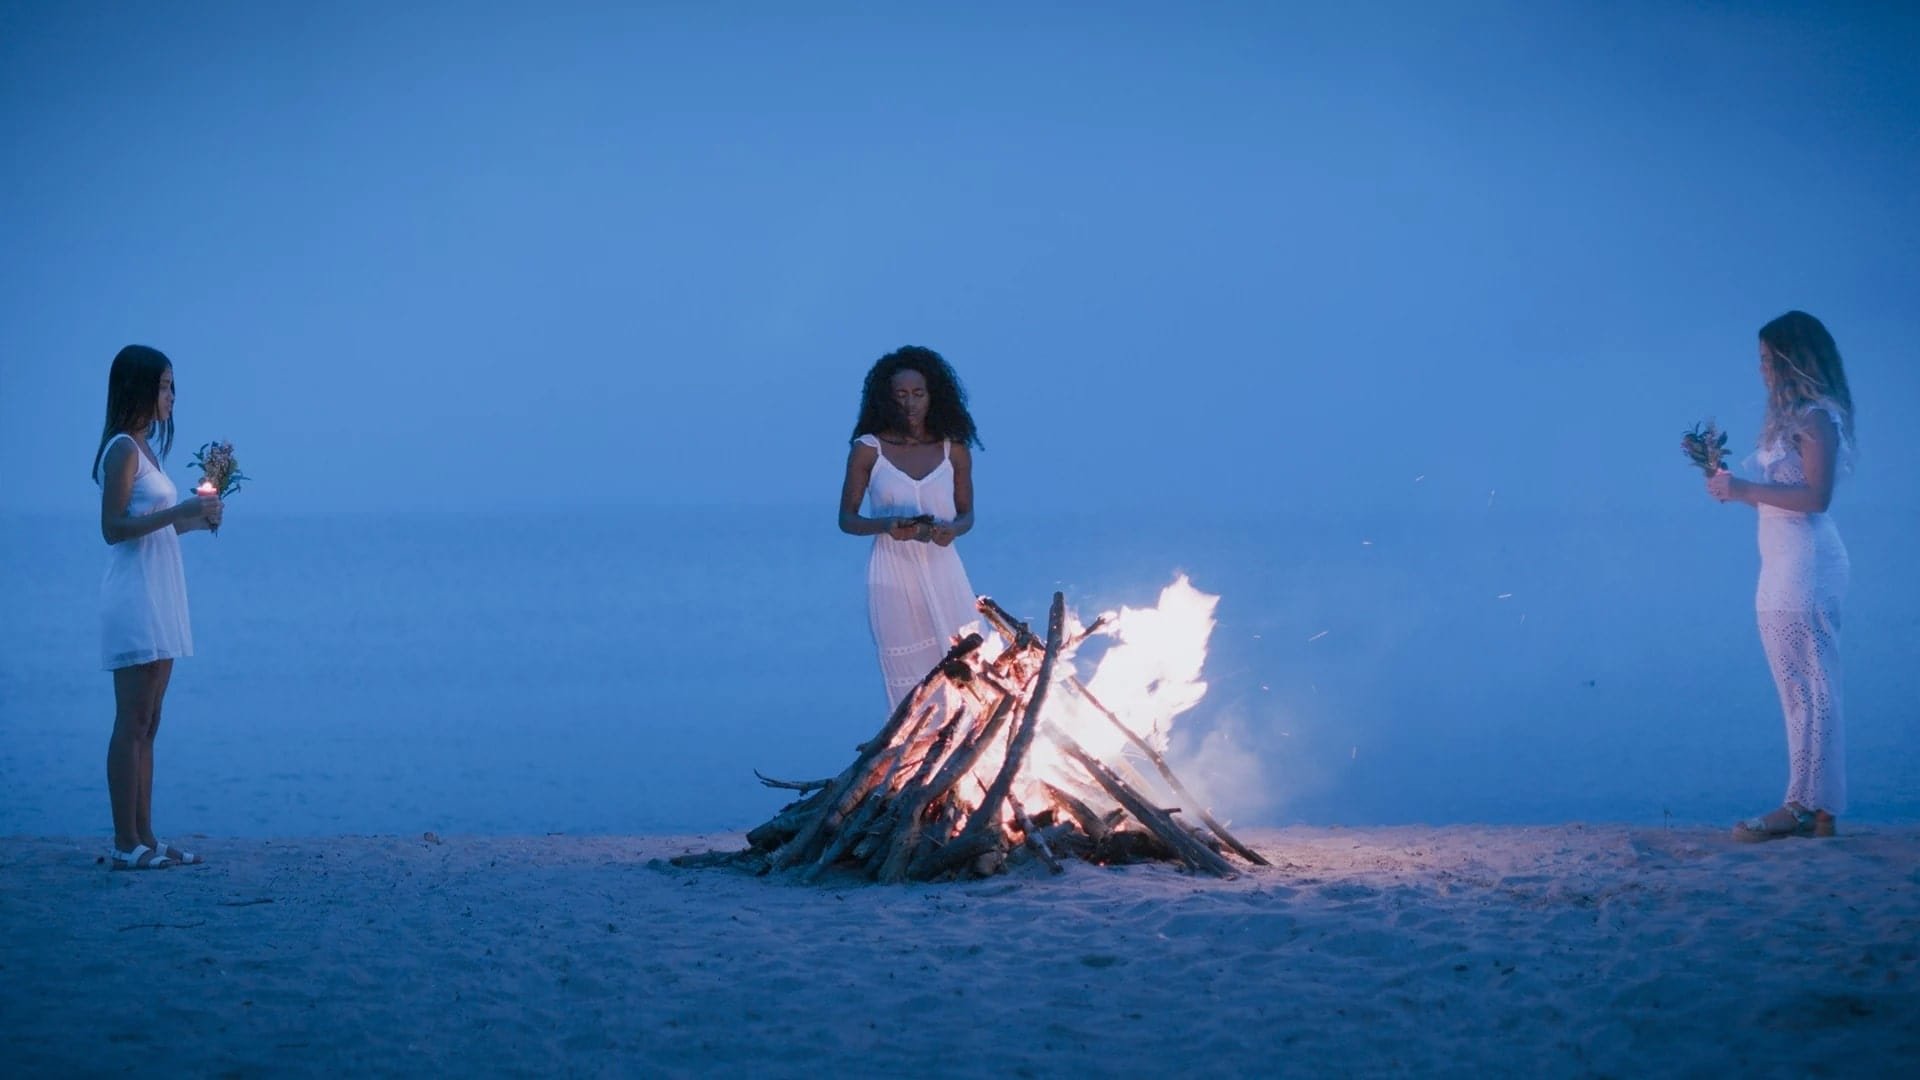
\includegraphics[width=0.5\textwidth]{imagens/SiempreBruja.jpg} \end{center}
\legend{Fonte: (Netflix, 2017)} \end{figure}


\subsection{\textit{The Ghost of a Tale}} Segundo o site do jogo (\citeyear{Ghostofa36:online})  ``Você é Tilo,
um corajoso rato menestrel em uma arriscada missão para achar seu verdadeiro
amor. Use sua furtividade e destreza para explorar o Forte \textit{Dwindling
Heights}''

\begin{figure}[!htb] \caption{\label{tale}The Ghost of a Tale} \begin{center}
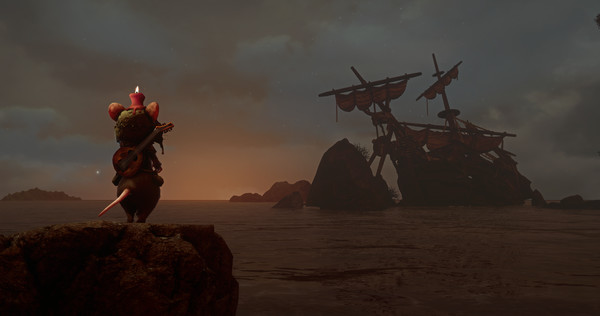
\includegraphics[width=0.5\textwidth]{imagens/tale.jpg} \end{center}
\legend{Fonte: \cite{Ghostofa36:online}} \end{figure}

\subsection{\textit{Moss}}
Em Moss, você ajuda o pequeno roedor Quill, a passar por muitos desafios para salvar seu tio. \cite{Moss18}

\begin{figure}[!htb] \caption{\label{fig_moss}Moss} \begin{center}
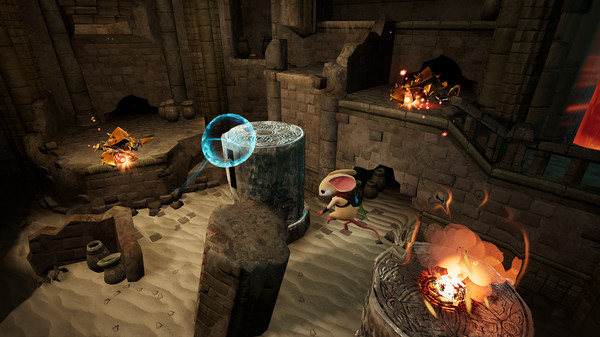
\includegraphics[width=0.5\textwidth]{imagens/moss.jpg} \end{center}
\legend{Fonte: \cite{Moss18}} \end{figure}


\subsection{\textit{Zelda: Windwaker}}

\section{Equipe de Desenvolvimento}

\subsection{Logo}

\subsection{Slogan}

\subsection{Divisão de tarefas}

A equipe dividiu-se de forma a
otimizar as forças de cada um dos integrantes, desta forma ficamos com a
seguinte divisão de tarefas não rígidas:

\begin{quadro}[htb] \caption{\label{quadro_atuacao}Atuação da equipe}
    \begin{tabularx}{\textwidth}{|c|X|} \hline \textbf{Nome} &
        \textbf{Atuação}\\ \hline Marina & Game Design Construção de
        Personagens, Construção de mundo, Design de personagens, Arte Conceitual
        \\ \hline Eric   & Construção de Personagens, Construção de mundo, Arte
        Técnica, Programação                                        \\ \hline
        Pedro  & Construção de Personagens, Construção de mundo, Arte Técnica,
        Programação \\ \hline \end{tabularx} \fonte{Própria autoria}
\end{quadro}
